\subsection{Experimento 1}

Instrumental utilizado:

\begin{itemize}
    \item Fuente lineal regulada de 0V a 15V.
    \item Multímetro Digital MMD BRYMEN BM-837 RS.
    \item Multímetro analógico Univo Elektronik.
\end{itemize}


Para este primer experimento se plantea realizar el circuito presentado a continuación en la figura \ref{fig:circuitoexp1}. 

\begin{figure}[H]
    \centering
    \begin{circuitikz} [scale=1,american, transform shape]
\def\scal{1};
\draw (0,-2) to[V,invert] (0,2)--(2,2) to[switch] (6,2) to[rmeterwa, t=V, v=\footnotesize{$Patron$},o-o] (6,-2)--(0,-2);
\draw (3,2)
    to[vR,o-o] (3,-2);
\draw (6,2)to[short,o-](8,2) to[smeter, t=V, v^=\footnotesize{$Contrastado$}] (8,-2)to[short,-o](6,-2);
\end{circuitikz}
    \caption{Circuito experimento 1}
    \label{fig:circuitoexp1}
\end{figure}

El experimento consiste en realizar un barrido de tensiones en un rango determinado y analizar las diferencias en las mediciones del instrumento patrón con respecto al instrumento contrastado. El multímetro digital será utilizado como instrumento patrón, mientras que el analógico será el instrumento contrastado. 

Para elegir el instrumento patrón se debe verificar que el error absoluto máximo del mismo se al menos 5 veces menor que el error absoluto máximo del contrastado. Para esto, se debe utilizar el dato de "clase" del multímetro contrastado (analógico) y despejando el error absoluto máximo de la fórmula de clase:

\begin{equation}\label{eq::clase}
    Clase= \frac{|\Delta V_{MAX}|}{Valor fiduciario}\cdot 100\%
\end{equation}

\begin{equation}
    |\Delta V_{MAX}|= \frac{Clase \cdot Valor fiduciario}{100\%}
\end{equation}

Reemplazando los valores queda:

\begin{equation}
    |\Delta V_{MAX}|= \frac{2.5\% \cdot 10[V]}{100\%}= 250[mV]
\end{equation}

Por lo que el instrumento patrón debe tener como máximo un error absoluto de 50 mV (un quinto del valor del instrumento contrastado). 

Se elige un fondo de escala adecuado en el multímetro patrón para realizar las mediciones. En este caso se eligió $40V$ como valor de fondo.
\clearpage
Según la hoja de datos, la expresión del error especificada para esa escala es:

\begin{equation}\label{eq::errorPatron}
    error_{patron} = 0.08\% + 1\; digitos
\end{equation}

Como la cifra menos significativa mostrada de acuerdo a la resolución del visor, es del orden de los 0.01 V, se debe sumar 10 mV al valor proporcional de cada error. En base a esto se calcula el máximo error absoluto posible en esa escala (40 V):

\begin{equation}
    error_{patron} = \frac{0.08\% \cdot 40 [V]}{100\%} + 10 [mV] = 42 [mV]
\end{equation}

De esta forma, se verifica que el multímetro digital es 5 veces más preciso que el analógico mediante el siguiente cálculo:

\begin{equation}
    \frac{|\Delta V_{MAX}|_{patron}}{error_{patron}} = 5.95
\end{equation}


Se debe seleccionar también un fondo de escala adecuado para el multímetro analógico. El valor elegido fue de 10 voltios, de manera que el barrido de tensiones pueda realizarse en el rango de 0 a 10 voltios. Luego se realiza la calibración del instrumento de medición analógico. Para ello se realizó una medición de 0 voltios y se situó la aguja indicadora correctamente en 0.

A continuación se comienza con el barrido de tensiones, poniendo a la aguja indicadora en cada uno de los valores de tensión correspondientes a su escala, y anotando el valor medido por el instrumento patrón (multímetro digital). Se aplicaron dos pasadas, una hacia arriba y otra hacia abajo y se anota el mayor error absoluto en cada índice entre ambas pasadas, como se puede observar en la Tabla \ref{tab:exp1a}.


\begin{table}[H]
    \centering
    \scalebox{0.9}{
    \begin{tabular}{|c||c|c|c|c|c|c|c|c|c|c|c|c|c|c|c|}
    \hline
         $V_L [V]$ & 1 & 2 & 3 & 4 & 5 & 6 & 7 & 8 & 9 & 10 \\
    \hline
        $V_p [V]$ (pasada hacia arriba) & 0.93 & 1.89 & 2.88 & 3.88 & 4.85 & 5.87 & 6.86 & 7.87 & 8.86 & 9.77  \\
    \hline
        $V_p [V]$ (pasada hacia abajo) & 0.94 & 1.88 & 2.86 & 3.87 & 4.85 & 5.86 & 6.86 & 7.86 & 8.86 & 9.79\\
    \hline
        $\Delta V [V]$ (mayor valor) & 0.07 & 0.12 & 0.14 & 0.13 & 0.15 & 0.14 & 0.14 & 0.14 & 0.14 & 0.23\\
         
    \hline
        \end{tabular}}
        \def\tablename{Tabla} 
        \caption{Mediciones del instrumento patrón y el mayor error absoluto}
        \label{tab:exp1a}
\end{table}

\begin{figure}[h!]
        \centering        
        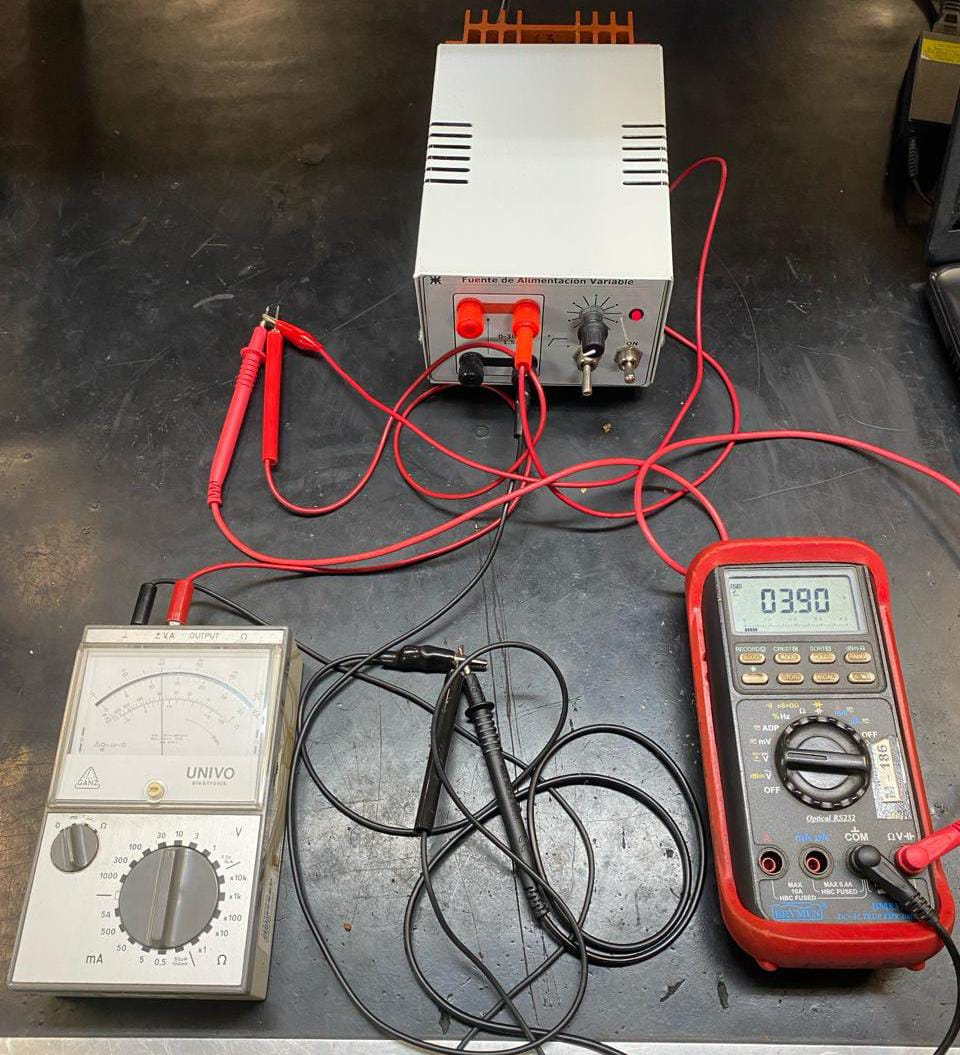
\includegraphics[width=0.35\textwidth]{Imagenes/Exp2.jpeg}
        \caption{Contrastación de un multímetro analógico con uno digital}
        \label{fig:contrast}
\end{figure}

\clearpage
 En base a los datos tabulados se confecciona la gráfica de corrección para representar cómo varia las mediciones con respecto al instrumento patrón. Sera útil para el usuario en caso de que quiera corregir de manera aproximadas el valor de su medición.

%FALTA lo de SUMAR y RESTAR en el grafico
%???

\begin{table}[H]
    \centering
    \scalebox{0.9}{
    \begin{tabular}{|c||c|c|c|c|}
    \hline
         & Instrumento constrastado & Patrón & Fecha & Operador \\
    \hline
        & Marca: Univo Elektronik & \makecell{Marca: UNI-T \\ Nro: UTC33C} & 26/03/2024 & Lucas Musso\\
    \hline
         &
        \multicolumn{4}{|c|}{
            %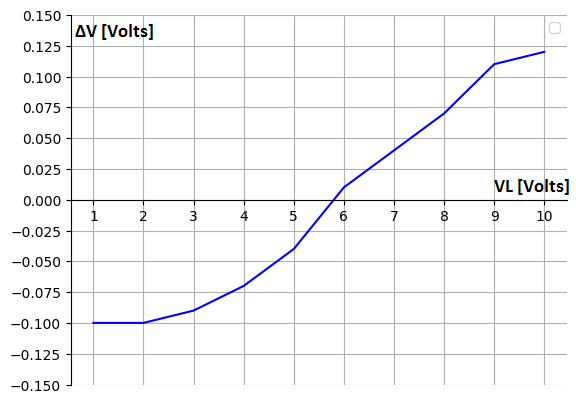
\includegraphics[width=\linewidth]{Imagenes/Grafica de correccion.png}
            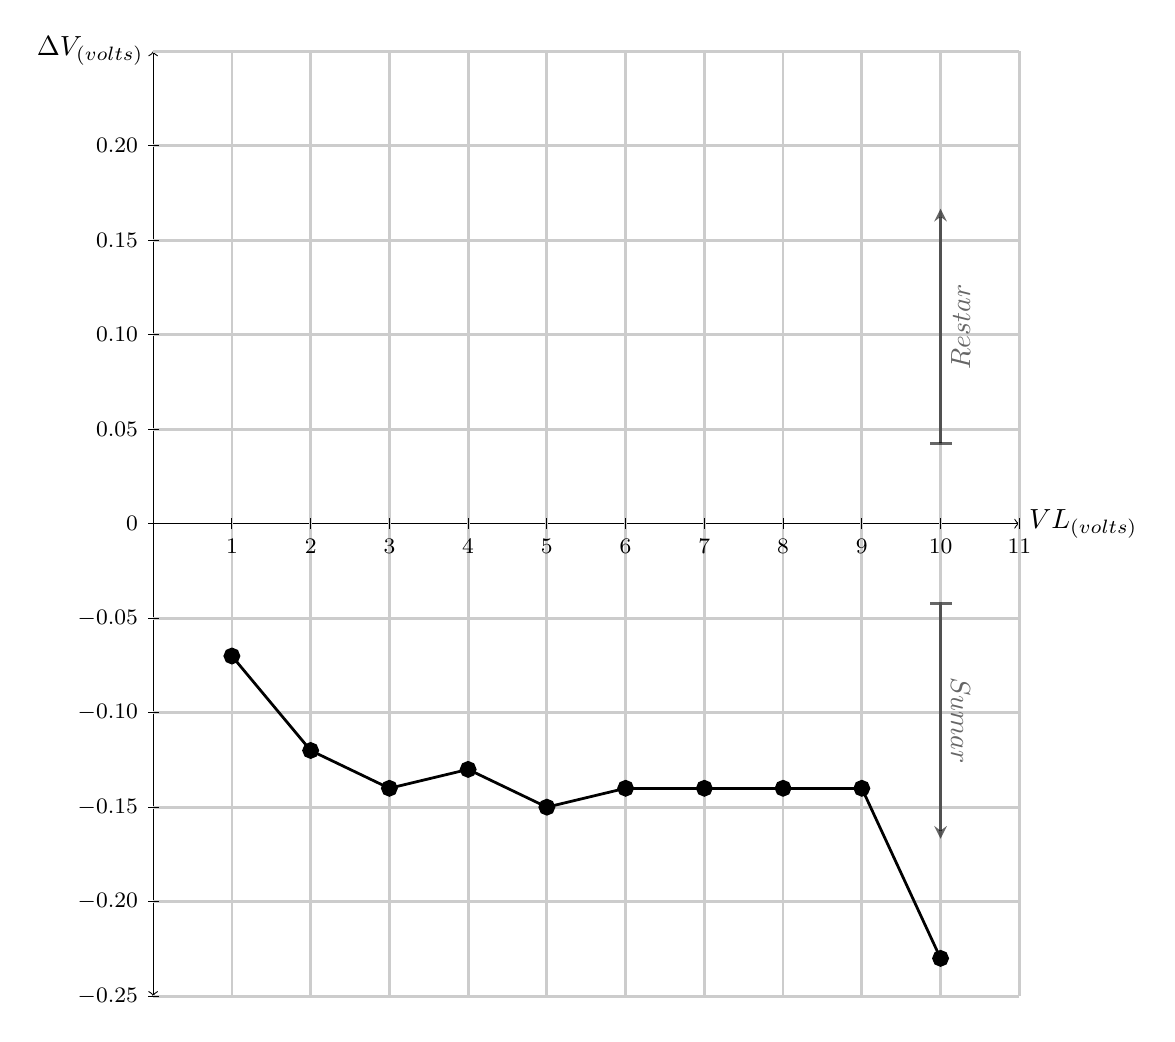
\begin{tikzpicture}[scale=1]
    
    \def\scal{6/0.25}
    
    %datosLineaA
    \coordinate (a1) at (1,-0.07*\scal);
    \coordinate (a2) at (2,-0.12*\scal);
    \coordinate (a3) at (3,-0.14*\scal);
    \coordinate (a4) at (4,-0.13*\scal);
    \coordinate (a5) at (5,-0.15*\scal);
    \coordinate (a6) at (6,-0.14*\scal);
    \coordinate (a7) at (7,-0.14*\scal);
    \coordinate (a8) at (8,-0.14*\scal);
    \coordinate (a9) at (9,-0.14*\scal);
    \coordinate (a10) at (10,-0.23*\scal);

    
    %Ejex
    \draw[->] (0,0)--(11,0) node[right] {$VL_{(volts)}$};
    \foreach \x in {1,2,...,11}{
        \draw[line width=1pt,gray!40] (\x,-6)--(\x,6);
        \draw[shift={(\x,0)}] (0pt,2pt) -- (0pt,-2pt) node[below] {\footnotesize $\x$};
    }
    %Ejey
    \draw[<->] (0,-6)--(0,6) node[left]{$\Delta V_{(volts)}$};;
    \foreach \y in {-0.25,-0.20,-0.15,-0.10,-0.05,0.05,0.10,0.15,0.20}{
        \draw[line width=1pt,gray!40] (0,\y*6/0.25)--(11,\y*6/0.25);
        \draw[shift={(0,\y*6/0.25)}] (2pt,0pt) -- (-2pt,0pt) node [left] {\footnotesize $\y$} ;
    }
   \draw[shift={(0,0)}] (2pt,0pt) -- (-2pt,0pt) node [left] {\footnotesize $0$} ;
   \draw[line width=1pt,gray!40] (0,6)--(11,6);
   
    %Linea A
    \foreach \x  in {1,...,10}{
        \draw[line width=2pt,fill=black] (a\x) circle(2pt);
   }
   \foreach \x [evaluate={\y=int(\x+1);}] in {1,...,9}{
        \draw[line width=1pt,black] (a\x) -- (a\y);
   }
   \draw[line width=1pt,opacity=0.6,|-stealth] (10,-1)--(10,-4) node[midway,sloped,above]{$Sumar$};
   \draw[line width=1pt,opacity=0.6,|-stealth] (10,1)--(10,4) node[midway,sloped,below]{$Restar$};
   
\end{tikzpicture}


        } \\
        
         
    \hline
        \end{tabular}}
        \def\tablename{Tabla} 
        \caption{Mediciones del instrumento patrón y el máximo error absoluto}
        \label{tab:exp1b}
\end{table}


Se puede obtener la clase de exactitud del instrumento analógico a partir del máximo error absoluto medido (0.23 V para el experimento) a partir de la ecuación \ref{eq::clase}

\begin{equation}
    Clase= \frac{0.23 [V]}{10 [V]} \cdot 100\% = 2.3\%
\end{equation}

El "valor fiduciario" es también conocido como fondo de escala, y es el máximo valor medible en esa configuración del instrumento.

Por lo tanto, tiene coherencia con la clase especificada en la hoja de datos del instrumento, la cual es 2.5\%

Una vez calculada la clase del multímetro analógico, se procede a analizar cuan precisas son las mediciones del instrumento digital con respecto a las del instrumento de contraste. Para ello se realiza el cálculo de la relación de error::

\begin{equation}
    Relacion\;error = \frac{\Delta V_{MAX}}{error_{patron}} \ge 5
\end{equation}

Como ya se dijo antes, la relación de error debe ser mayor a 5 para toda la escala del instrumento patrón. Se puede representar la relación Medición - Error absoluto en una tabla para verificar hasta que esta condición se cumple (Tabla \ref{tab:relacionerror})

\begin{table}[h!]
    \centering
    \scalebox{0.99}{
    \begin{tabular}{|c||c|c|}
    \hline
         Medición & Error patrón & Relación error \\ \hline
        1   &  0.0108  &  21.30 \\ \hline
        2  &  0.0116  &  19.83 \\ \hline
        3  &  0.0124  &  18.55 \\ \hline
        4  &  0.0132  &  17.42 \\ \hline
        5  &  0.0140  &  16.43 \\ \hline
        6  &  0.0148  &  15.54 \\ \hline
        7  &  0.0156  &  14.74 \\ \hline
        8  &  0.0164  &  14.02 \\ \hline
        9  &  0.0172  &  13.37 \\ \hline
        10 &  0.0180  &  12.78 \\ \hline
        \end{tabular}}
        \def\tablename{Tabla} 
        \caption{Relaciones de errores entre instrumento patrón y de contraste}
        \label{tab:relacionerror}
\end{table}

\begin{figure}[H]
    \centering
    \begin{tikzpicture}[scale=1]
\def\scal{6/10}
\def\des{12}
    
    %datosLineaA
    \coordinate (a1) at (1,21.3*\scal-\des*\scal);
    \coordinate (a2) at (2,19.83*\scal-\des*\scal);
    \coordinate (a3) at (3,18.55*\scal-\des*\scal);
    \coordinate (a4) at (4,17.42*\scal-\des*\scal);
    \coordinate (a5) at (5,16.43*\scal-\des*\scal);
    \coordinate (a6) at (6,15.54*\scal-\des*\scal);
    \coordinate (a7) at (7,14.74*\scal-\des*\scal);
    \coordinate (a8) at (8,14.02*\scal-\des*\scal);
    \coordinate (a9) at (9,13.37*\scal-\des*\scal);
    \coordinate (a10) at (10,12.78*\scal-\des*\scal);

    %Ejex
    \draw[->] (0,0)--(11,0) node[midway,below={5mm}] {Medición};
    \foreach \x in {0,1,2,...,11}{
        \draw[line width=1pt,gray!40] (\x,0) -- (\x,6);
        \draw[shift={(\x,0)}] (0pt,2pt) -- (0pt,-2pt) node[below] {\footnotesize $\x$};
    }
    %Linea A
    \foreach \c in {1,...,10}{
        \draw[line width=1pt,gray!40] let \p1 = (a\c)in (11,\y1)--(0,\y1);
        \draw[] let \p1= (a\c)in (2pt,\y1) -- (-2pt,\y1);
   }
    \foreach \x  in {1,...,10}{
        \draw[line width=2pt,fill=black] (a\x) circle(1pt);
   }
   \foreach \x [evaluate={\y=int(\x+1);}] in {1,...,9}{
        \draw[line width=1pt,black] (a\x) -- (a\y);
   }

   
    %Ejey
    \draw[->] (0,0)--(0,6) node[midway,sloped,above={15mm}]{Relación error};
    \foreach \c in {1,2,4,6,10}{
        
    }
    
   \draw[] let \p1= (a1)in (2pt,\y1) -- (-2pt,\y1) node[left] {\footnotesize $21.30$};
   \draw[] let \p1= (a2)in (2pt,\y1) -- (-2pt,\y1) node[left] {\footnotesize $19.83$};
   \draw[] let \p1= (a3)in (2pt,\y1) -- (-2pt,\y1) node[left] {\footnotesize $18.55$};
   \draw[] let \p1= (a4)in (2pt,\y1) -- (-2pt,\y1) node[left] {\footnotesize $17.42$};
   \draw[] let \p1= (a5)in (2pt,\y1) -- (-2pt,\y1) node[left] {\footnotesize $16.43$};
   \draw[] let \p1= (a6)in (2pt,\y1) -- (-2pt,\y1) node[left] {\footnotesize $15.54$};
   \draw[] let \p1= (a7)in (2pt,\y1) -- (-2pt,\y1) node[left] {\footnotesize $14.74$};
   \draw[] let \p1= (a8)in (2pt,\y1) -- (-2pt,\y1) node[left] {\footnotesize $14.02$};
   \draw[] let \p1= (a9)in (2pt,\y1) -- (-2pt,\y1) node[left] {\footnotesize $13.37$};
   \draw[] let \p1= (a10)in (2pt,\y1) -- (-2pt,\y1) node[left] {\footnotesize $12.78$};

 
\end{tikzpicture}
    \caption{Relaciones de errores entre instrumento patrón y de contraste}
    \label{fig:relacionerror}
\end{figure}




